\documentclass[11pt,a4paper]{article}
\usepackage[T1]{fontenc}\usepackage[utf8]{inputenc}\usepackage{lmodern,microtype,amsmath,amssymb,amsthm,mathtools,bm,booktabs,array,tabularx,longtable,graphicx,float,caption,xcolor,enumitem,fancyhdr,hyperref}
\usepackage[margin=22mm]{geometry}
\definecolor{finblue}{HTML}{1F5A99}\definecolor{fingreen}{HTML}{19733A}\definecolor{finorange}{HTML}{C45A00}\definecolor{finred}{HTML}{A61B1B}\definecolor{finsoft}{HTML}{F2F5F8}
\hypersetup{colorlinks=true,linkcolor=finblue,urlcolor=finblue,pdftitle={FIN ST642--ST731: Current-Strict Causal-Physics No-Go and Minimal Conditional 3+1 Maxwell Bridge},pdfauthor={Krzysztof Żuchowski},pdfsubject={Six FIN research rounds on continuum, Lorentz, gauge, dimension, clocks and operational falsification},pdfkeywords={FIN, causality, Lorentz, Maxwell, photon, refinement, no-go theorem, conditional bridge}}
\pagestyle{fancy}\fancyhf{}\fancyhead[L]{FIN ST642--ST731}\fancyhead[R]{Release 10.91}\fancyfoot[C]{\thepage}\setlength{\headheight}{14pt}
\newtheorem{theorem}{Theorem}[section]\newtheorem{corollary}[theorem]{Corollary}
\newcommand{\status}[2]{\textcolor{#1}{\textbf{[#2]}}}\newcommand{\proven}{\status{fingreen}{PROVEN}}\newcommand{\strong}{\status{finblue}{STRONG EVIDENCE}}\newcommand{\conditional}{\status{finorange}{CONDITIONAL}}\newcommand{\blocked}{\status{finred}{BLOCKED}}
\newcommand{\claimbox}[1]{\begin{center}\fcolorbox{finblue}{finsoft}{\parbox{.92\textwidth}{#1}}\end{center}}
\setlist[itemize]{leftmargin=*,itemsep=2pt}\setlength{\emergencystretch}{2em}
\begin{document}\hypersetup{pageanchor=false}
\begin{titlepage}\centering\vspace*{14mm}{\Huge\bfseries FIN ST642--ST731\par}\vspace{4mm}{\Large Current-Strict Causal-Physics No-Go\par}{\Large and the Minimal Conditional $3+1$ Maxwell Bridge\par}\vspace{12mm}{\Large Krzysztof Żuchowski\par}{\normalsize Independent Researcher --- Fractal Information Theory Project\par}{\normalsize ORCID: 0009-0002-0909-3613\par}\vspace{9mm}{\large Six consecutive research rounds\par}{\large FIN Release 10.91 --- Version 1.0.0\par}{\large 30 August 2026\par}\vfill
\begin{minipage}{.91\textwidth}\small\textbf{Scope.} This report continues the verified ST552--ST641 propagation programme. It asks whether the conditional scalar light cone can be upgraded to strong continuum dynamics, $3+1$ isotropy, Lorentz-compatible dispersion, Maxwell kinematics, photon structure and an operational test.

\medskip\textbf{Evidence boundary.} Results are analytic, finite, conditional or explicitly numerical. No independent laboratory or external-review record is introduced. Legacy physical roles are not transferred.\end{minipage}\vfill\end{titlepage}\hypersetup{pageanchor=true}

\begin{abstract}
Six further FIN research rounds, ST642--ST731, investigate whether the previously constructed conditional scalar wave cone can become an inevitable $3+1$ causal-light theory. The answer is a theorem-level no-go for the present strict core together with a minimal conditional bridge.

Uniform fixed-range locality plus exact scale-shift self-similarity conditionally forces the zero antipodal-rate tower, but neither premise is strict-sourced. Complete coarse Green, unitary and heat data remain constant on the refinement-speed fiber and cannot select it. On fixed Fourier bands the conditional wave propagators converge strongly. A threefold Cartesian product yields leading isotropic symbol $C|\mathbf k|^2$ and lattice anisotropy/boost defects of order $a^2$. A supplied cubic cochain complex realizes exact Abelian gauge kinematics, Maxwell-type energy, Gauss constraint, two transverse directions and Maxwell dispersion. Yet the scalar Laplacian admits infinitely many gauge-complex extensions and does not select spatial dimension, electric/magnetic coefficients, helicity or photon quantization.

Three conditional physics principles intersect at $3+1$: conformal invariance of the Maxwell 2-form action selects four spacetime dimensions, two transverse polarizations select three spatial dimensions, and the minimal sharp Huygens dimension is three. Their agreement is coherent but imports the very Maxwell/polarization/Huygens premises whose provenance is sought.

The final architecture contains seven explicitly distinct packages: refinement/coordinate law $R$, two clock classes $T$, dimension/carrier $D$, gauge/Maxwell data $G$, independent calibration $C$, operational instruments/records $O$, and state/orientation sector $S$. Removing each restores an explicit nonidentifiability or no-go. Therefore the current strict spectral core cannot uniquely export causal-light physics. A richer strict nadsoliton source may evade this theorem, but no such source is present. A complete calibration-invariant model-discrimination library and fail-closed transfer schema are supplied; no laboratory evidence follows.
\end{abstract}
\tableofcontents\newpage

\section{Executive theorem}
\claimbox{\textbf{Main conclusion.} Current FIN can construct a coherent causal-wave/Maxwell theory only conditionally. The strict endpoint and all present coarse spectral/Green data are invariant on nontrivial fibers of refinement speed, spatial dimension, gauge complex, clock scaling, calibration and orientation. No invariant deterministic map from those data can uniquely choose observed causal-light physics.}

The minimal bridge is
\[
\boxed{A_{12}+R+T+D+G+C+O+S.}
\]
Here $R$ selects a local refinement and coordinate embedding; $T$ supplies diffusive and ballistic clocks; $D$ supplies a $3$-dimensional carrier; $G$ supplies an edge/face complex and Maxwell coefficients; $C$ supplies noncircular units; $O$ supplies state-to-record operations; and $S$ supplies a realized orientation/helicity when needed.

\section{Round I: ST642--ST656}
Uniform fixed-range locality forbids every sufficiently fine antipodal rate $q_N$. If the same local rule is required at every dyadic scale, it forces $q_N=0$ at all levels. This selects the local tower only after adding locality and exact scale-shift self-similarity.

On a fixed Fourier band, rescaled wave frequencies converge uniformly. Extended finite-grid tails outside $1.05ct$ fall below $5\times10^{-14}$ at $N=24576$, although a uniform analytic tail theorem remains open.

A conditional threefold product gives leading $3$-dimensional isotropic symbol. Axis/diagonal anisotropy decreases from $4.49\times10^{-2}$ at $a=.25$ to $7.45\times10^{-4}$ at $a=.03125$.
\begin{figure}[H]\centering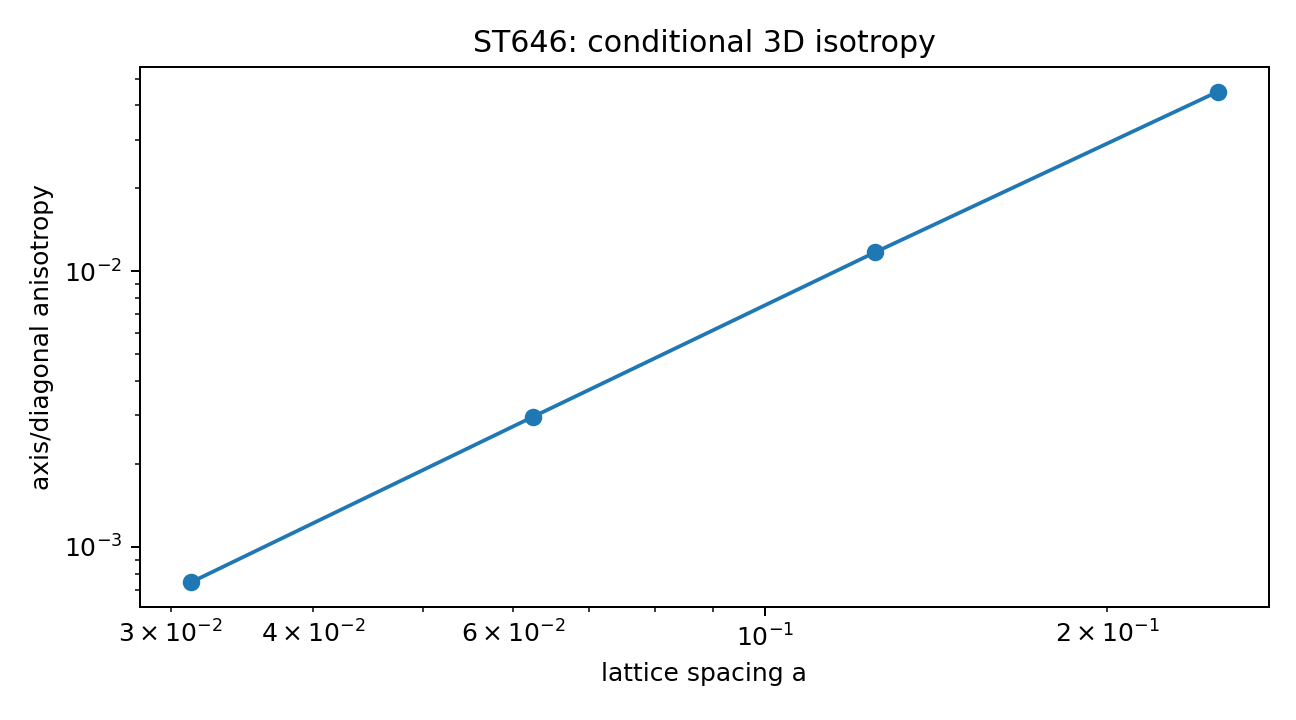
\includegraphics[width=.78\textwidth]{FIN_ST642_ST656_Figures/st646_isotropy.png}\caption{Conditional cubic anisotropy vanishes as $O(a^2)$.}\end{figure}

The scalar endpoint does not determine a vector/one-form module, exterior complex, gauge connection, Gauss constraint or polarizations. A signed refinement with a negative stiffness mode is dynamically unstable in raw heat and second-order wave channels.

\begin{longtable}{@{}p{.1\textwidth}p{.29\textwidth}p{.5\textwidth}@{}}\toprule Program&Status&Result\\\midrule\endhead
ST642--643&\proven&Conditional locality selection; coarse Green selector no-go.\\
ST644--647&\proven/\strong&Band convergence, tail evidence, 3D isotropy and $O(a^2)$ boost defect.\\
ST648&\proven&Scalar-to-gauge nonuniqueness.\\
ST649--650&\strong/\proven&Two-clock identification and noncircular anchor requirement.\\
ST651--652&\proven&Polynomial direct tails and signed instability.\\
ST653&\strong&Affine IR predictor improves residuals by factor $\sim480$.\\
ST654--656&blocked&Independent mathematical/source/evidence gates remain closed.\\\bottomrule\end{longtable}

\section{Round II: ST657--ST671}
Conditional $3$-dimensional product propagators converge on fixed bands, while finite-spacing boost defects fall by a factor near $1/4$ under halving $a$. A supplied cubic complex has 27 vertices, 81 edges and 81 faces with exact
\[
d_1d_0=0.
\]
It gives Abelian gauge transformations $A\mapsto A+d_0\phi$ and invariant field strength $F=d_1A$.

The same scalar $d_0^*d_0$ admits inequivalent edge/face extensions. Hodge decomposition of the fixture has 26 gradient directions, 52 curl directions and 3 harmonic zero modes. These sectors are not contained in the scalar endpoint.

\begin{figure}[H]\centering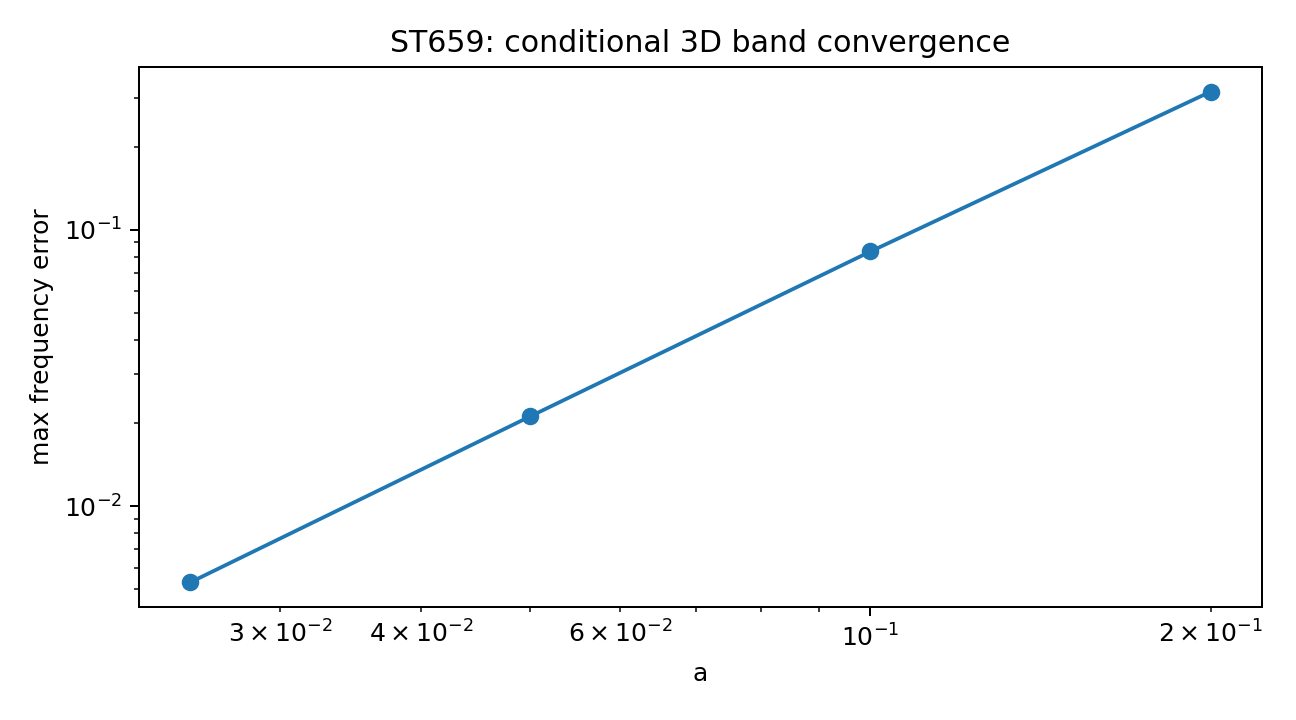
\includegraphics[width=.78\textwidth]{FIN_ST657_ST671_Figures/st659_3d_convergence.png}\caption{Conditional $3$D band-limited wave convergence.}\end{figure}

Synthetic two-clock regression with 1\% log noise estimates exponents $1.99996$ and $0.999998$ with zero ordering errors in 2,000 replicates. This is methodological readiness, not clock evidence.

\section{Round III: ST672--ST686}
Every product dimension $D\ge1$ contains the same one-axis scalar dynamics. Fine heat traces can identify $D$, but complete one-axis coarse records cannot.

A supplied Maxwell Hamiltonian
\[
H=\frac12\left(\kappa_E\|E\|^2+\kappa_B\|B\|^2\right)
\]
is gauge invariant and preserves Gauss when initialized in $\ker d_0^*$. Its cubic transverse dispersion is
\[
\omega^2=\frac4{a^2}\sum_i\sin^2\frac{ak_i}{2}\longrightarrow|\mathbf k|^2.
\]
Every nonzero $3$D wave vector has two transverse directions.

\begin{figure}[H]\centering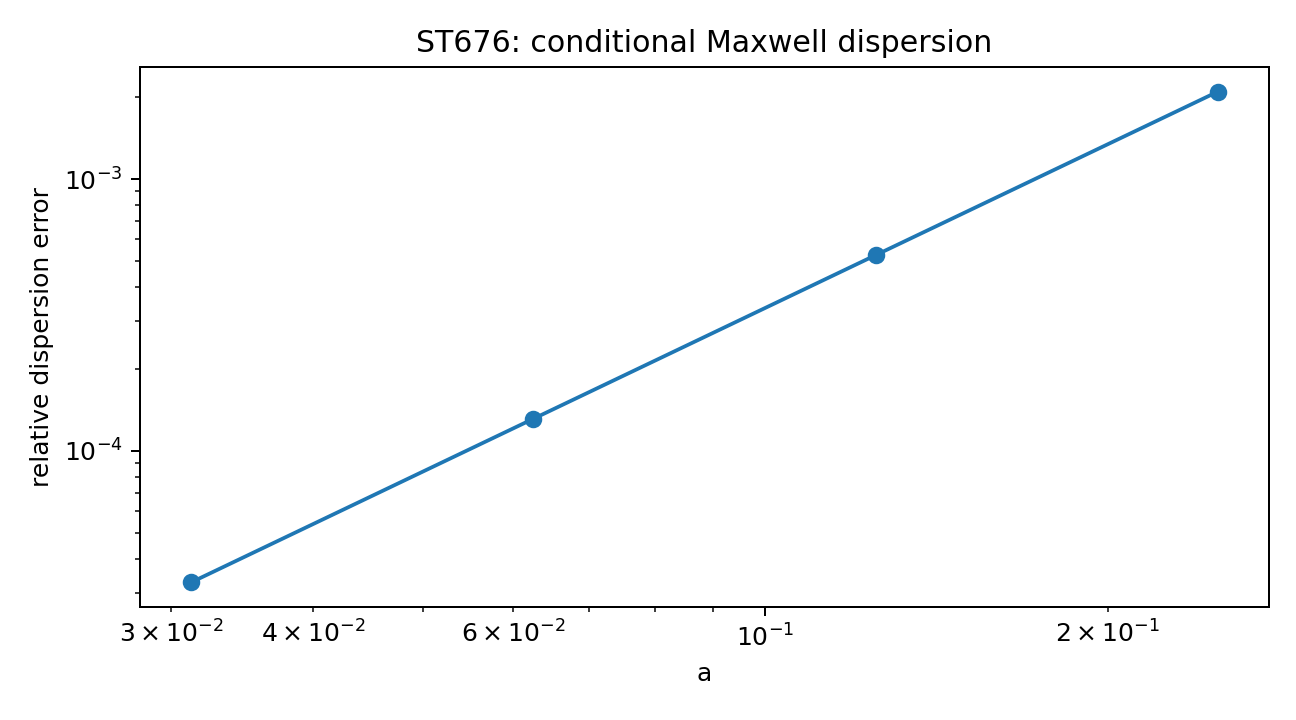
\includegraphics[width=.78\textwidth]{FIN_ST672_ST686_Figures/st676_maxwell_dispersion.png}\caption{Conditional cubic Maxwell dispersion.}\end{figure}

The coefficients remain moduli:
\[
c_{\rm gauge}=\sqrt{\kappa_E\kappa_B}\,\widehat c,
\qquad Z=\sqrt{\kappa_E/\kappa_B}.
\]
Neither their values, gauge coupling, charge unit, $\hbar$, photon Fock representation nor helicity selector follows from $A_{12}$.

\section{Round IV: ST687--ST701}
Three conditional selectors converge on $3+1$:
\begin{enumerate}
\item Maxwell action $\int F\wedge*F$ scales under $g\mapsto\Omega^2g$ as $\Omega^{n-4}$, hence is conformal at spacetime dimension $n=4$.
\item A massless vector in $D$ spatial dimensions has $D-1$ transverse polarizations; two select $D=3$.
\item The smallest nontrivial spatial dimension with sharp Huygens propagation for the standard massless wave equation is $D=3$.
\end{enumerate}
\begin{figure}[H]\centering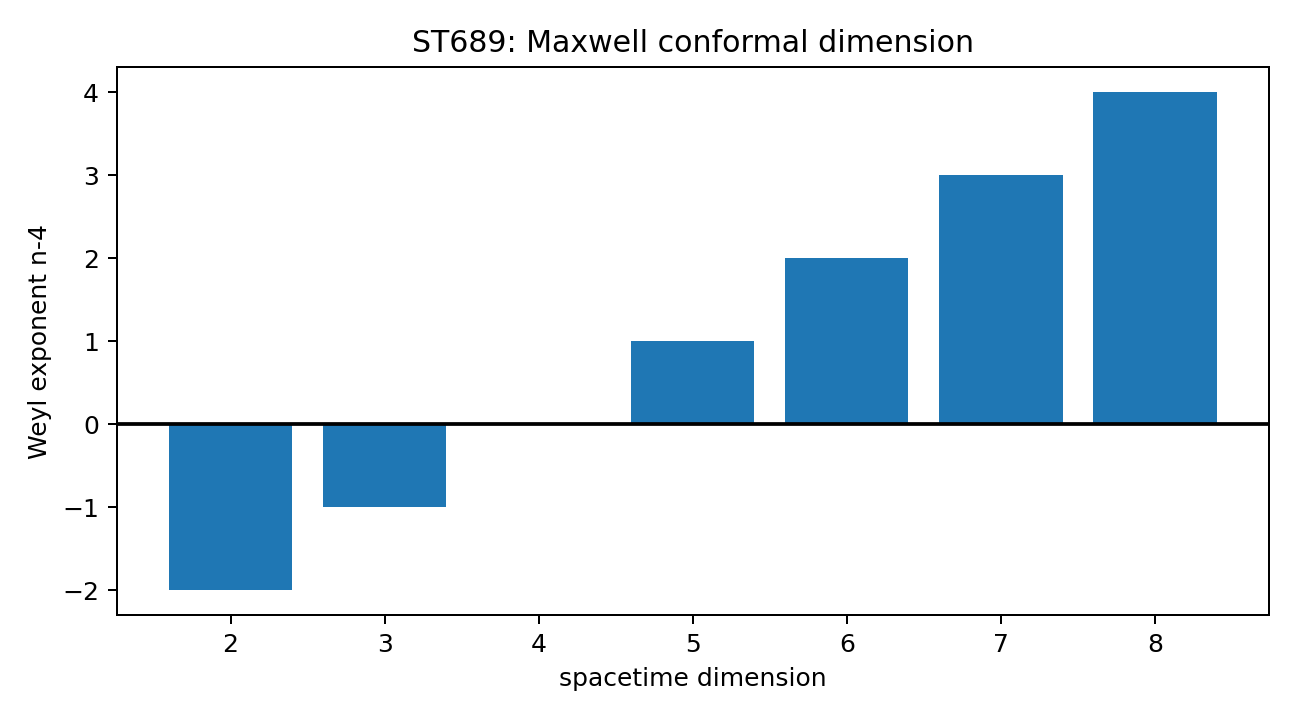
\includegraphics[width=.76\textwidth]{FIN_ST687_ST701_Figures/st689_conformal_dimension.png}\caption{Classical Maxwell conformal scaling selects four spacetime dimensions conditionally.}\end{figure}
These principles are imported physical axioms. Their intersection is not strict provenance.

Classical transverse modes still require a complex structure/positive-frequency split, commutators, $\hbar$, vacuum, Fock representation and Born instruments before they are photons. A parity-even radial kernel cannot choose helicity sign.

\section{Round V: ST702--ST716}
A six-model library was frozen: local scalar models in $D=1,2,3$, a local $D=3$ gauge model, a fractional $D=3$ scalar model and an unstable signed model. Ideal features were
\[
(D,\nu,\text{polarizations},\text{Gauss},\text{stability},\text{tail class},\text{clock classes}).
\]
The exact minimum-cardinality separating feature sets were enumerated. A synthetic noisy classifier has total error below 1\%, and a hidden fractional model excluded from the candidate library is flagged as out-of-library.

Fail-closed schemas require independent rod and clock identifiers, hashes fixed before wave unblinding, two distinct clock slopes, raw multilevel records and provider/registrar/analyst separation. Software cannot generate independent custody.

\begin{figure}[H]\centering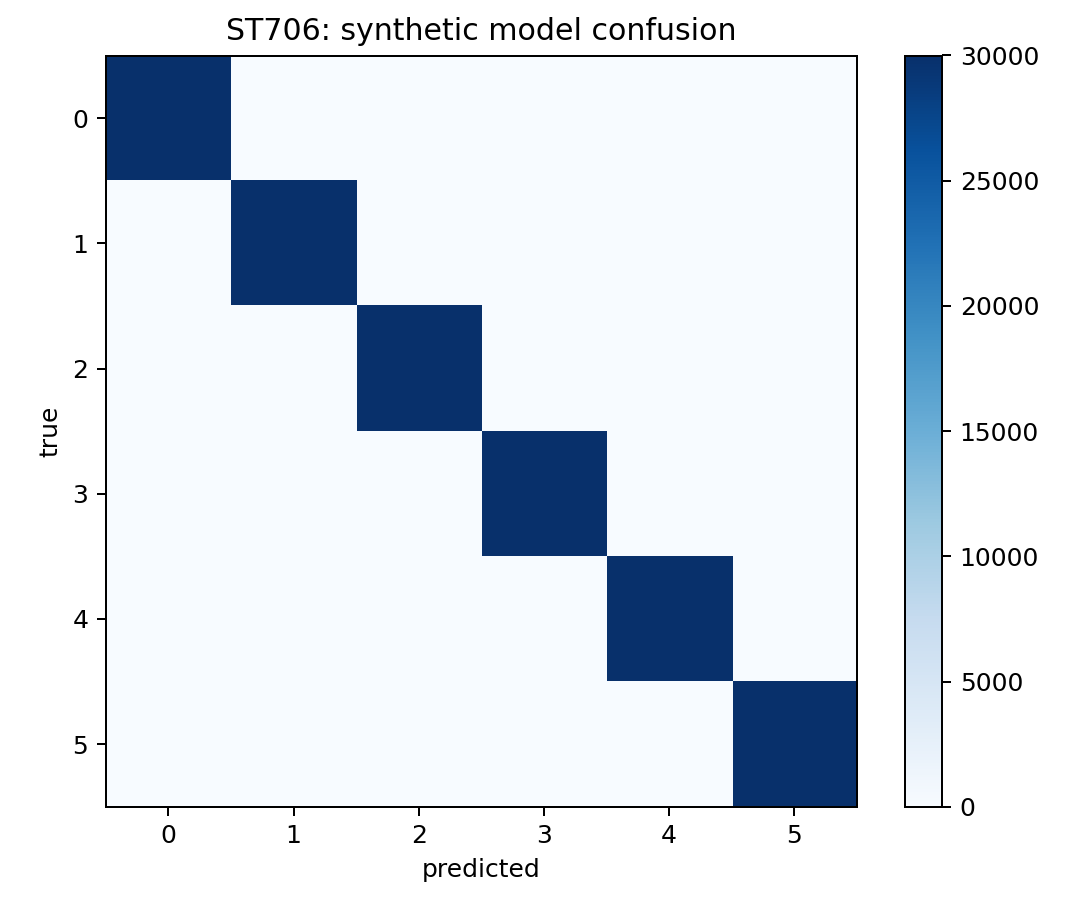
\includegraphics[width=.68\textwidth]{FIN_ST702_ST716_Figures/st706_confusion.png}\caption{Synthetic model-library confusion matrix.}\end{figure}

\section{Round VI: ST717--ST731}
\subsection{Minimal bridge and axiom removal}
The final typed bridge contains seven packages:
\begin{longtable}{@{}p{.08\textwidth}p{.34\textwidth}p{.48\textwidth}@{}}\toprule Package&Content&Loss when removed\\\midrule\endhead
$R$&zero-rate local refinement and coordinates&continuous speed fiber; no selected continuum\\
$T$&diffusive $a^{-2}$ and ballistic $a^{-1}$ clocks&single-clock no-go\\
$D$&three-dimensional carrier&dimension product fiber\\
$G$&edge/face complex and Maxwell coefficients&scalar wave only; no gauge/polarizations\\
$C$&independent dimensional calibration&no SI-valued prediction\\
$O$&preparations, instruments, apparatus, records&no map to empirical events\\
$S$&state/orientation/helicity sector&no canonical realized sign or branch\\\bottomrule\end{longtable}

\begin{theorem}[Current-strict causal-physics no-go]
No deterministic construction invariant under all presently established strict equivalences can uniquely export a physical causal-light theory from the finite radial spectral core. At least one of $R,T,D,G,C,O,S$ must add a source, break a demonstrated fiber, or provide missing operational data.
\end{theorem}
The theorem is not an absolute no-go for all future FIN. A richer strict nadsoliton object outside the audited equivalence classes may export one or more packages.

\subsection{Conditional predictions}
Conditioned on the bridge, the model predicts
\[
\omega^2=C|\mathbf k|^2+O(a^2k^4),\quad
\text{anisotropy and boost defect}=O(a^2),\quad
2\text{ transverse modes},\quad d_0^*E=0,
\]
together with clock exponents $(2,1)$ and sharply different local/fractional/signed causal tails. These are falsifiable model predictions, not strict constants of nature.

\section{Falsification and final status}
\begin{longtable}{@{}p{.3\textwidth}p{.28\textwidth}p{.32\textwidth}@{}}\toprule Proposed inference&Obstruction&Status\\\midrule\endhead
$A_{12}\Rightarrow$ unique refinement&exact $q$ fiber&refuted in current class\\
coarse Green data $\Rightarrow q$&all coarse functions constant on fiber&refuted\\
scalar Laplacian $\Rightarrow$ gauge complex&infinite harmonic/cell extensions&refuted\\
scalar records $\Rightarrow D=3$&all product dimensions share restriction&refuted\\
one clock for all channels&exponents $2$ and $1$&refuted\\
two polarizations $\Rightarrow D=3$&valid only after vector/light premise&conditional\\
conformal Maxwell $\Rightarrow3+1$&imports Maxwell action&conditional\\
conditional bridge $\Rightarrow$ nature&no independent record&blocked\\\bottomrule\end{longtable}

\claimbox{\textbf{Final verdict.} FIN now possesses a precise conditional route from a finite informational operator to local scalar waves and a coherent $3+1$ Maxwell scaffold. It does not possess a theorem making that route inevitable. The missing physical principle must source or select refinement, two clocks, dimension, gauge complex, calibration, operations and state/orientation sectors.}

\section{Recommended next cycle: ST732--ST746}
\begin{enumerate}
\item strict locality/source theorem for the zero-rate tower;
\item full-energy wave convergence and a uniform cone-tail proof;
\item source or obstruction for a $3$D carrier and Lorentz representation;
\item gauge-complex and Maxwell-coefficient provenance;
\item photon quantization and helicity interface;
\item physical two-clock apparatus and noncircular anchor transfer;
\item nuisance-robust model-library tests;
\item predictor-correlated IR intervals;
\item transition/algebra method gates;
\item strict-source and independent-evidence gates.
\end{enumerate}

\appendix
\section{Reproducibility}
The authoritative sequence runs from \path{FIN_ST642_ST656_Results.json} through \path{FIN_ST717_ST731_Results.json}, with six Python sources, six summaries, figures and tests. The combined suite covers all 90 packet hashes and principal theorem/nonpromotion flags.

\section{Nonclaims}
No laboratory result, external referee, legacy-to-strict completion, legacy role transfer, strict selector, physical SI speed, photon, Standard Model, gravity, $L_{\rm total}$ or ToE closure follows. All future PDFs remain English.
\end{document}
